\begin{pastexam}[label={px:ntust-111-et-ds-06}]{臺科大電子所甲組 111 學年度 第 6 題}
（追蹤）

(25\%) Consider the graph $G$.
\begin{enumerate}[label=(\arabic*)]
\item Show its adjacency matrix. (5\%)
\item Show its adjacency list. (5\%)
\item Show the depth-first spanning tree starting from node 0 based on your adjacency list in (2). (5\%)
\item Show the breadth-first spanning tree starting from node 0 based on your adjacency list in (2). (5\%)
\item Find a minimum spanning tree using Kruskal's algorithm. (5\%)
\end{enumerate}
\begin{center}
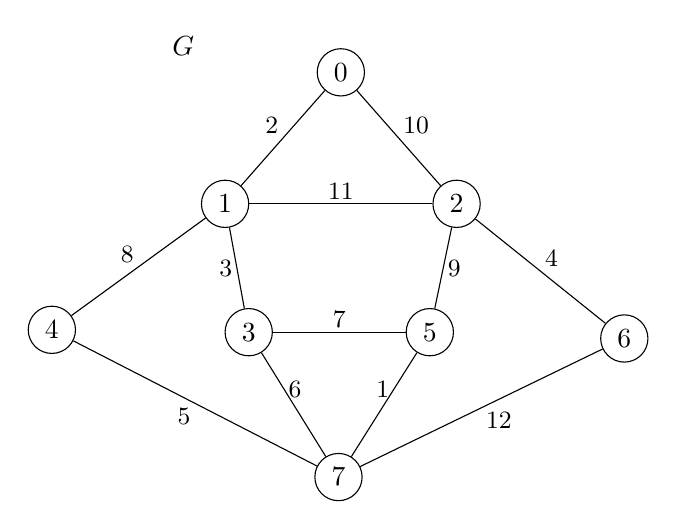
\begin{tikzpicture}[v/.style={circle,draw,inner sep=1.5pt,minimum size=6mm},w/.style={font=\small,inner sep=1.5pt}]
\node[v] (n0) at (22.00,-1.13) {0};
\node[v] (n1) at (20.53,-2.80) {1};
\node[v] (n2) at (23.47,-2.80) {2};
\node[v] (n4) at (18.33,-4.40) {4};
\node[v] (n3) at (20.83,-4.43) {3};
\node[v] (n5) at (23.13,-4.43) {5};
\node[v] (n6) at (25.60,-4.51) {6};
\node[v] (n7) at (21.97,-6.27) {7};
\draw[] (n0) -- node[w,above left] {2} (n1);
\draw[] (n0) -- node[w,above right] {10} (n2);
\draw[] (n1) -- node[w,above] {11} (n2);
\draw[] (n1) -- node[w,above left] {8} (n4);
\draw[] (n1) -- node[w,left] {3} (n3);
\draw[] (n2) -- node[w,right] {9} (n5);
\draw[] (n2) -- node[w,above right] {4} (n6);
\draw[] (n3) -- node[w,above] {7} (n5);
\draw[] (n3) -- node[w,right,pos=0.35] {6} (n7);
\draw[] (n5) -- node[w,left,pos=0.35] {1} (n7);
\draw[] (n4) -- node[w,below left] {5} (n7);
\draw[] (n6) -- node[w,below right] {12} (n7);
\node at (20.00,-0.80) {$G$};
\end{tikzpicture}
\end{center}
\end{pastexam}

\begin{pastsoln}
(1)--(4) 屬資結書第~21~章；(5) 屬第~24~章。 $G$ 是無向加權圖，$8$ 個頂點、$12$ 條邊。

\textbf{(1) 鄰接矩陣}（資結書第~21.2~節）。 $A[i][j] = 1$ 表示 $i$、$j$ 之間有邊；無向圖的矩陣對稱。 左邊是只記
有沒有邊的矩陣；因為 $G$ 有權重，也可以寫成右邊的成本矩陣（有邊記權重，沒有邊記 $\infty$，對角線記 $0$）。
\begin{center}
\small
\begin{tabular}{c|*{8}{c}}
 & 0 & 1 & 2 & 3 & 4 & 5 & 6 & 7 \\ \hline
0 & 0 & 1 & 1 & 0 & 0 & 0 & 0 & 0 \\
1 & 1 & 0 & 1 & 1 & 1 & 0 & 0 & 0 \\
2 & 1 & 1 & 0 & 0 & 0 & 1 & 1 & 0 \\
3 & 0 & 1 & 0 & 0 & 0 & 1 & 0 & 1 \\
4 & 0 & 1 & 0 & 0 & 0 & 0 & 0 & 1 \\
5 & 0 & 0 & 1 & 1 & 0 & 0 & 0 & 1 \\
6 & 0 & 0 & 1 & 0 & 0 & 0 & 0 & 1 \\
7 & 0 & 0 & 0 & 1 & 1 & 1 & 1 & 0 \\
\end{tabular}
\qquad
\begin{tabular}{c|*{8}{c}}
 & 0 & 1 & 2 & 3 & 4 & 5 & 6 & 7 \\ \hline
0 & 0 & 2 & 10 & $\infty$ & $\infty$ & $\infty$ & $\infty$ & $\infty$ \\
1 & 2 & 0 & 11 & 3 & 8 & $\infty$ & $\infty$ & $\infty$ \\
2 & 10 & 11 & 0 & $\infty$ & $\infty$ & 9 & 4 & $\infty$ \\
3 & $\infty$ & 3 & $\infty$ & 0 & $\infty$ & 7 & $\infty$ & 6 \\
4 & $\infty$ & 8 & $\infty$ & $\infty$ & 0 & $\infty$ & $\infty$ & 5 \\
5 & $\infty$ & $\infty$ & 9 & 7 & $\infty$ & 0 & $\infty$ & 1 \\
6 & $\infty$ & $\infty$ & 4 & $\infty$ & $\infty$ & $\infty$ & 0 & 12 \\
7 & $\infty$ & $\infty$ & $\infty$ & 6 & 5 & 1 & 12 & 0 \\
\end{tabular}
\end{center}

\textbf{(2) 鄰接串列}。 每個頂點一條串列，鄰居依編號由小到大排列（串列的順序會決定 (3)(4) 的答案，以下都照這個
順序）。 每個節點存鄰居和邊的權重；無向圖每條邊出現兩次，共 $24$ 個節點。
\begin{center}
\begin{tabular}{ll}
\toprule
頂點 & 鄰接串列（鄰居，邊的權重）\\
\midrule
0 & (1, 2) $\to$ (2, 10) $\to$ \NIL \\
1 & (0, 2) $\to$ (2, 11) $\to$ (3, 3) $\to$ (4, 8) $\to$ \NIL \\
2 & (0, 10) $\to$ (1, 11) $\to$ (5, 9) $\to$ (6, 4) $\to$ \NIL \\
3 & (1, 3) $\to$ (5, 7) $\to$ (7, 6) $\to$ \NIL \\
4 & (1, 8) $\to$ (7, 5) $\to$ \NIL \\
5 & (2, 9) $\to$ (3, 7) $\to$ (7, 1) $\to$ \NIL \\
6 & (2, 4) $\to$ (7, 12) $\to$ \NIL \\
7 & (3, 6) $\to$ (4, 5) $\to$ (5, 1) $\to$ (6, 12) $\to$ \NIL \\
\bottomrule
\end{tabular}
\end{center}

\textbf{(3) DFS 生成樹}（資結書第~21.4~節）。 從 $0$ 出發，每到一個頂點就照它的串列順序找第一個沒拜訪過的鄰居往下走，
沒有了才退回：
\begin{itemize}
\item $0 \to 1$（$0$ 的第一個鄰居）；$1$ 的鄰居 $0$ 已拜訪，走 $1 \to 2$；$2$ 的鄰居 $0, 1$ 已拜訪，走 $2 \to 5$；
$5$ 的鄰居 $2$ 已拜訪，走 $5 \to 3$；$3$ 的鄰居 $1, 5$ 已拜訪，走 $3 \to 7$；$7$ 的鄰居 $3$ 已拜訪，走 $7 \to 4$。
\item $4$ 的鄰居 $1, 7$ 都拜訪過，退回 $7$；$7$ 的下一個鄰居 $5$ 已拜訪，走 $7 \to 6$。
\item $6$ 的鄰居 $2, 7$ 都拜訪過；一路退回 $0$，所有頂點都拜訪過，結束。
\end{itemize}
拜訪順序 $0, 1, 2, 5, 3, 7, 4, 6$；樹邊 $(0,1), (1,2), (2,5), (5,3), (3,7), (7,4), (7,6)$。

\textbf{(4) BFS 生成樹}（資結書第~21.3~節）。 從 $0$ 出發，佇列依序處理，每個頂點把還沒拜訪的鄰居依串列順序放進佇列：
\begin{itemize}
\item 取出 $0$：放入 $1, 2$（樹邊 $(0,1), (0,2)$）。
\item 取出 $1$：$0, 2$ 已拜訪，放入 $3, 4$（樹邊 $(1,3), (1,4)$）。
\item 取出 $2$：$0, 1$ 已拜訪，放入 $5, 6$（樹邊 $(2,5), (2,6)$）。
\item 取出 $3$：$1, 5$ 已拜訪，放入 $7$（樹邊 $(3,7)$）。
\item 取出 $4, 5, 6, 7$：鄰居都已拜訪。
\end{itemize}
拜訪順序 $0, 1, 2, 3, 4, 5, 6, 7$；樹邊 $(0,1), (0,2), (1,3), (1,4), (2,5), (2,6), (3,7)$。

\textbf{(5) Kruskal}（資結書第~24.2~節，虛擬碼~24.2）。 邊依權重由小到大處理，兩端不在同一棵樹（不會形成環）就加入：
\begin{center}
\begin{tabular}{cll}
\toprule
邊 & 權重 & 結果 \\
\midrule
$(5,7)$ & 1 & 加入 \\
$(0,1)$ & 2 & 加入 \\
$(1,3)$ & 3 & 加入 \\
$(2,6)$ & 4 & 加入 \\
$(4,7)$ & 5 & 加入 \\
$(3,7)$ & 6 & 加入（把 $\{0,1,3\}$ 和 $\{4,5,7\}$ 接起來） \\
$(3,5)$ & 7 & 捨棄：$3$、$5$ 已經連通（$3$--$7$--$5$） \\
$(1,4)$ & 8 & 捨棄：$1$--$3$--$7$--$4$ 已連通 \\
$(2,5)$ & 9 & 加入（把 $\{2,6\}$ 接上），已有 $7$ 條邊，結束 \\
\bottomrule
\end{tabular}
\end{center}
最小生成樹的邊是 $(5,7), (0,1), (1,3), (2,6), (4,7), (3,7), (2,5)$，總權重 $1 + 2 + 3 + 4 + 5 + 6 + 9 = 30$。
所有邊的權重都不同，所以最小生成樹是唯一的。

下圖粗線是各小題的樹邊，灰色虛線是其他的邊：
\begin{center}
\begin{tikzpicture}[x=0.62cm,y=0.71cm,v/.style={circle,draw,inner sep=1pt,minimum size=5.5mm,font=\small},w/.style={font=\scriptsize,inner sep=1pt},te/.style={very thick},ne/.style={black!35,dashed}]
\node[v] (n0) at (0.00,-1.13) {0};
\node[v] (n1) at (-1.47,-2.80) {1};
\node[v] (n2) at (1.47,-2.80) {2};
\node[v] (n4) at (-3.67,-4.40) {4};
\node[v] (n3) at (-1.17,-4.43) {3};
\node[v] (n5) at (1.13,-4.43) {5};
\node[v] (n6) at (3.60,-4.51) {6};
\node[v] (n7) at (-0.03,-6.27) {7};
\draw[te] (n0) -- (n1);
\draw[ne] (n0) -- (n2);
\draw[te] (n1) -- (n2);
\draw[ne] (n1) -- (n4);
\draw[ne] (n1) -- (n3);
\draw[te] (n2) -- (n5);
\draw[ne] (n2) -- (n6);
\draw[te] (n3) -- (n5);
\draw[te] (n3) -- (n7);
\draw[ne] (n5) -- (n7);
\draw[te] (n4) -- (n7);
\draw[te] (n6) -- (n7);
\node[font=\small] at (0,-7.2) {(3) DFS 生成樹};
\end{tikzpicture}\hspace{0.5cm}\begin{tikzpicture}[x=0.62cm,y=0.71cm,v/.style={circle,draw,inner sep=1pt,minimum size=5.5mm,font=\small},w/.style={font=\scriptsize,inner sep=1pt},te/.style={very thick},ne/.style={black!35,dashed}]
\node[v] (n0) at (0.00,-1.13) {0};
\node[v] (n1) at (-1.47,-2.80) {1};
\node[v] (n2) at (1.47,-2.80) {2};
\node[v] (n4) at (-3.67,-4.40) {4};
\node[v] (n3) at (-1.17,-4.43) {3};
\node[v] (n5) at (1.13,-4.43) {5};
\node[v] (n6) at (3.60,-4.51) {6};
\node[v] (n7) at (-0.03,-6.27) {7};
\draw[te] (n0) -- (n1);
\draw[te] (n0) -- (n2);
\draw[ne] (n1) -- (n2);
\draw[te] (n1) -- (n4);
\draw[te] (n1) -- (n3);
\draw[te] (n2) -- (n5);
\draw[te] (n2) -- (n6);
\draw[ne] (n3) -- (n5);
\draw[te] (n3) -- (n7);
\draw[ne] (n5) -- (n7);
\draw[ne] (n4) -- (n7);
\draw[ne] (n6) -- (n7);
\node[font=\small] at (0,-7.2) {(4) BFS 生成樹};
\end{tikzpicture}\hspace{0.5cm}\begin{tikzpicture}[x=0.62cm,y=0.71cm,v/.style={circle,draw,inner sep=1pt,minimum size=5.5mm,font=\small},w/.style={font=\scriptsize,inner sep=1pt},te/.style={very thick},ne/.style={black!35,dashed}]
\node[v] (n0) at (0.00,-1.13) {0};
\node[v] (n1) at (-1.47,-2.80) {1};
\node[v] (n2) at (1.47,-2.80) {2};
\node[v] (n4) at (-3.67,-4.40) {4};
\node[v] (n3) at (-1.17,-4.43) {3};
\node[v] (n5) at (1.13,-4.43) {5};
\node[v] (n6) at (3.60,-4.51) {6};
\node[v] (n7) at (-0.03,-6.27) {7};
\draw[te] (n0) -- node[w,above left] {2} (n1);
\draw[ne] (n0) -- node[w,above right] {10} (n2);
\draw[ne] (n1) -- node[w,above] {11} (n2);
\draw[ne] (n1) -- node[w,above left] {8} (n4);
\draw[te] (n1) -- node[w,left] {3} (n3);
\draw[te] (n2) -- node[w,right] {9} (n5);
\draw[te] (n2) -- node[w,above right] {4} (n6);
\draw[ne] (n3) -- node[w,above] {7} (n5);
\draw[te] (n3) -- node[w,right,pos=0.35] {6} (n7);
\draw[te] (n5) -- node[w,left,pos=0.35] {1} (n7);
\draw[te] (n4) -- node[w,below left] {5} (n7);
\draw[ne] (n6) -- node[w,below right] {12} (n7);
\node[font=\small] at (0,-7.2) {(5) MST（總重 30）};
\end{tikzpicture}
\end{center}
\end{pastsoln}
